\frame{
    \frametitle{Contents}
    \begin{enumerate}
    \item About Me
        \vspace{0.5cm}
    \item Introduction to CODEX-b
        \vspace{0.5cm}
    \item Background measurement at LHCb cavern
        \vspace{0.5cm}
    \item Simulation with DD4hep
        \vspace{0.5cm}
    \item Summary and future plans
        \vspace{0.5cm}
    \end{enumerate}
}

\frame{
   \frametitle{About Me}
   \begin{columns}
   \column{0.5\textwidth}
   \centering
   \includegraphics[angle=-90,width=5cm]{pictures/myPhoto.jpg}
   \column{0.5\textwidth}
   \centering
   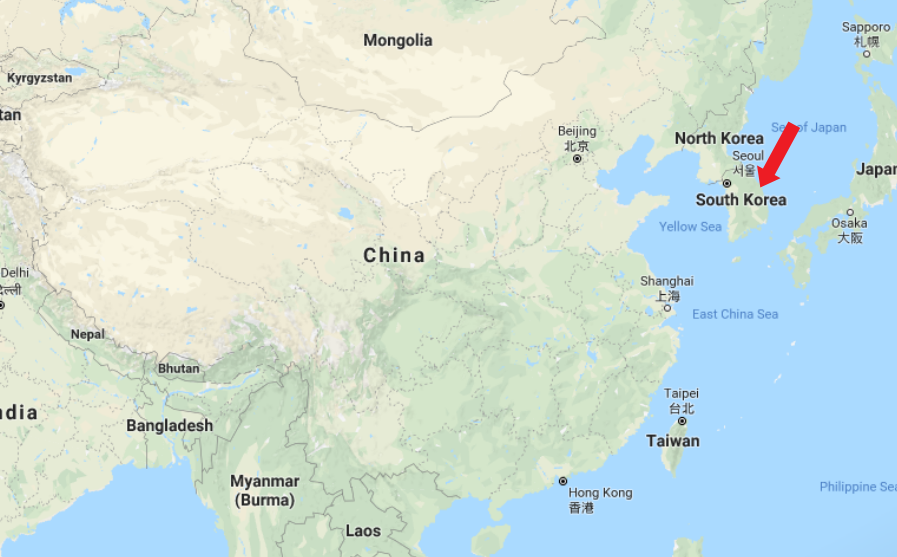
\includegraphics[width=5cm]{pictures/mymap.png}
   \begin{itemize}
    \item From South Korea (9,200 km)
      \vspace{0.3cm}
    \item Kyungpook National University, Daegu 
      \vspace{0.3cm}
    \item First year master course student in experimental high energy physics
   \end{itemize}
   \end{columns}
}

\frame{
    \frametitle{Long-lived particles (LLPs) at HL-LHC}
    \begin{itemize}
    \item No clear observation of new physics (NP) at the LHC as yet
    \vspace{0.3cm}
    \item NP portal: weakly coupled sector with long lifetime 
    \vspace{0.3cm}
    \item Long lifetimes very generic in any theory with multiple mass scales, broken symmetries... SM is a good example
    \end{itemize}
    \vspace{0.2cm}
    \begin{columns}
    \column{0.5\textwidth}
    \centering
        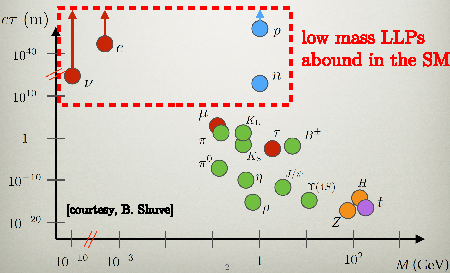
\includegraphics[width=5.5cm]{pictures/shuve_llp.pdf} \\
    \column{0.5\textwidth}
    \centering
        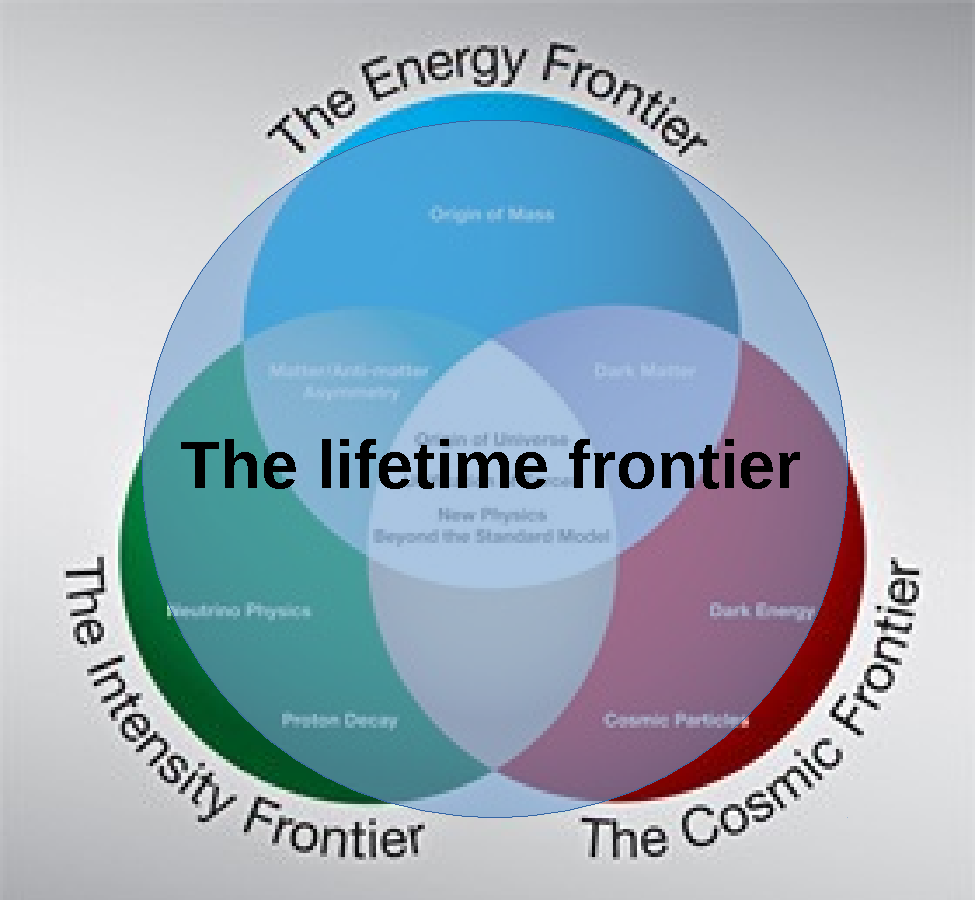
\includegraphics[width=3.8cm]{pictures/lifetime_frontier.pdf} \\
    \end{columns}
    %\item Existing detectors (ATLAS, CMS, LHCb) not optimized to find
    %\newline LLPs due to large QCD backgrounds and limited coverage
}

\frame{
    \frametitle{Other LLP detector proposals at the LHC}
   \begin{columns}
	\column{0.5\textwidth}
	\centering
    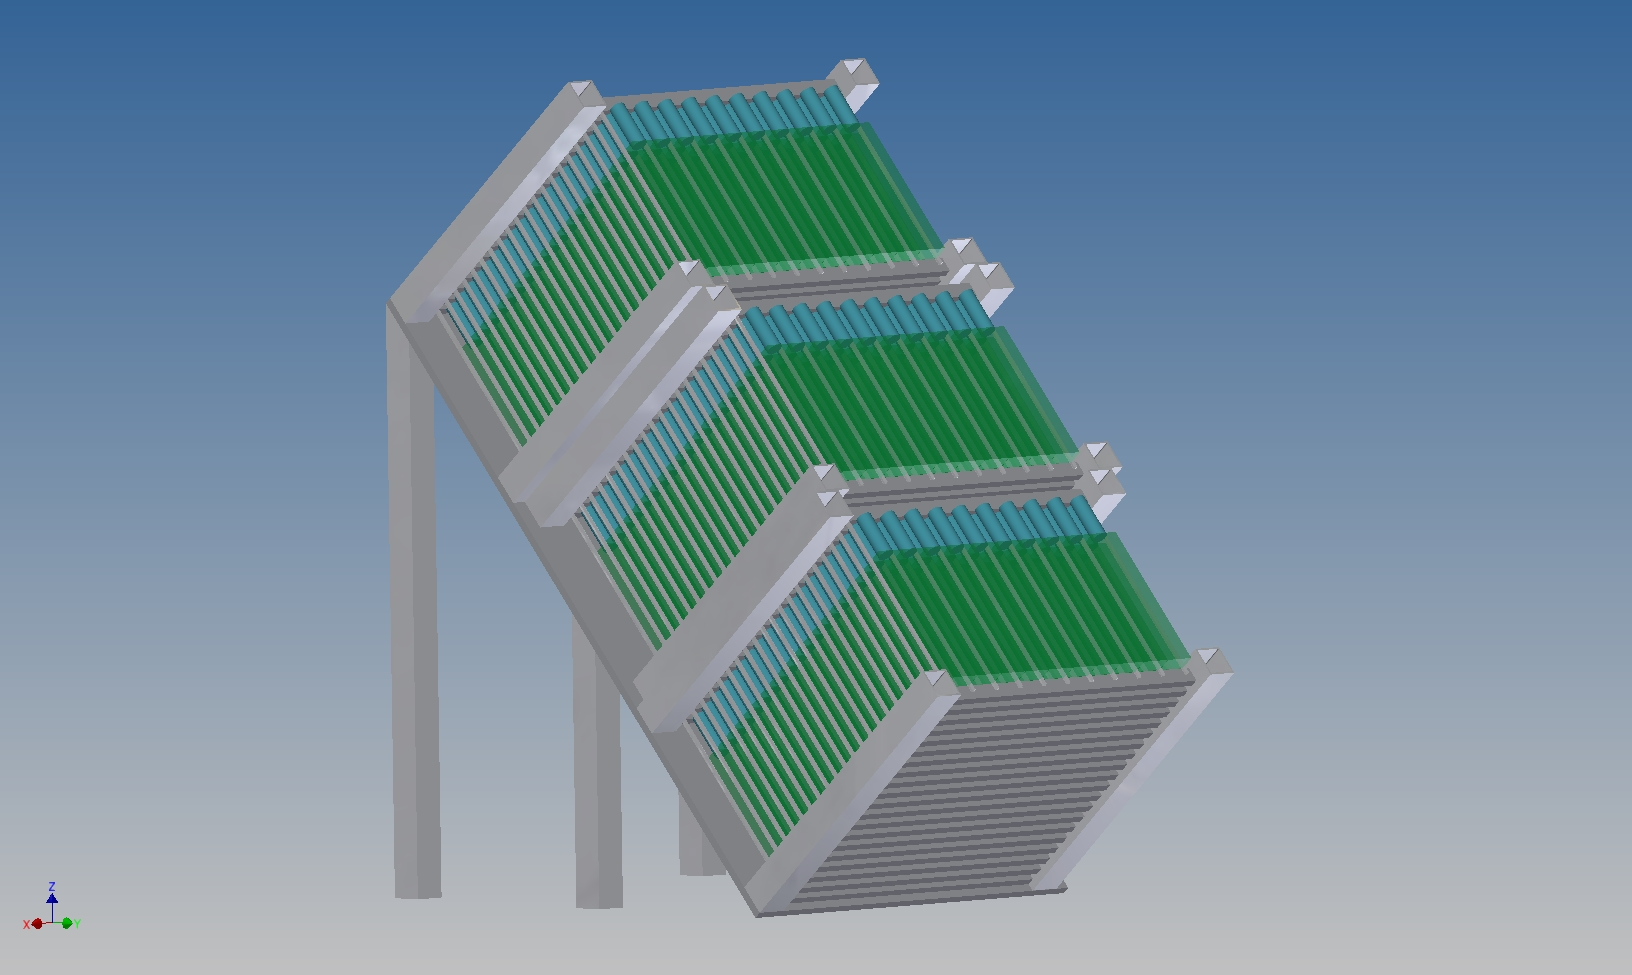
\includegraphics[width=1.9in]{pictures/milliqan}\\ {\tt MilliQan: \href{https://arxiv.org/abs/1607.04669}{\textcolor{blue}{1607.04669}}}
	\column{0.5\textwidth}
	\centering
	\vspace{-0.6cm}
	    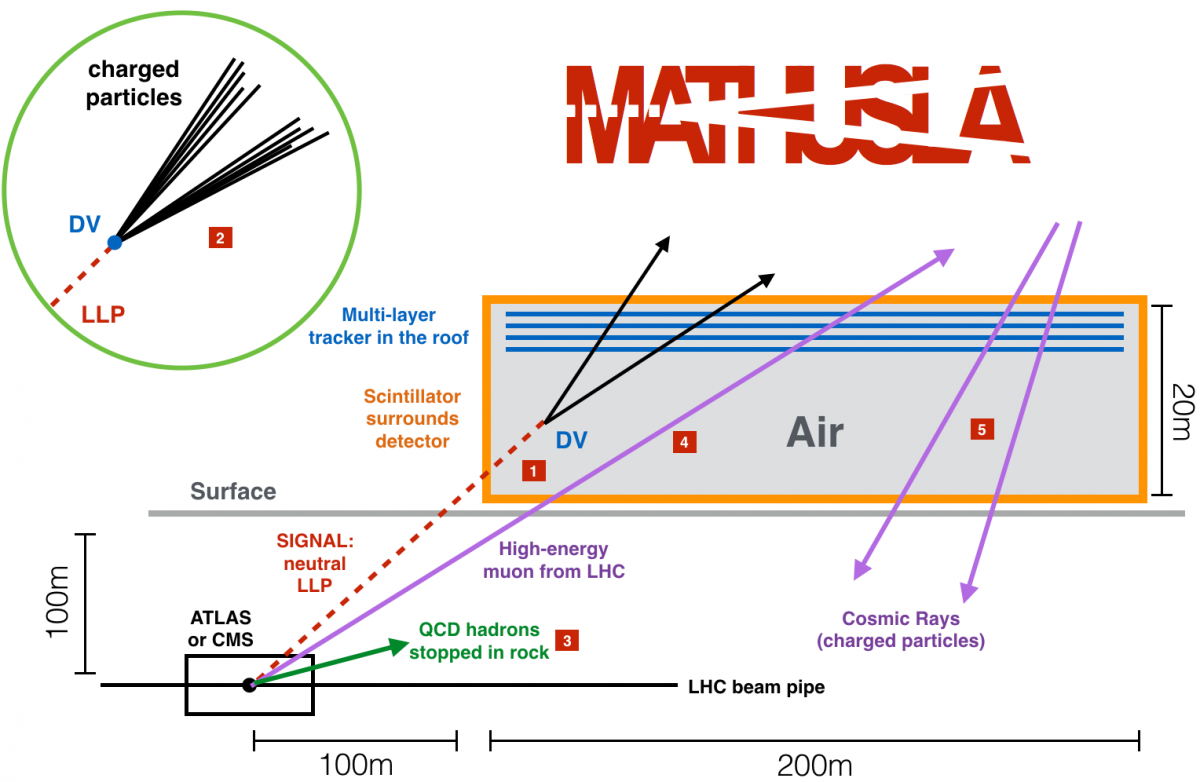
\includegraphics[width=1.9in]{pictures/mathusla}\\\vspace{0.4cm} {\tt MATHUSLA: \href{https://arxiv.org/abs/1606.06298}{\textcolor{blue}{1606.06298}}}
	\end{columns}
\vspace{0.5cm}
   \begin{columns}[T]
	\column{0.5\textwidth}
	\centering
	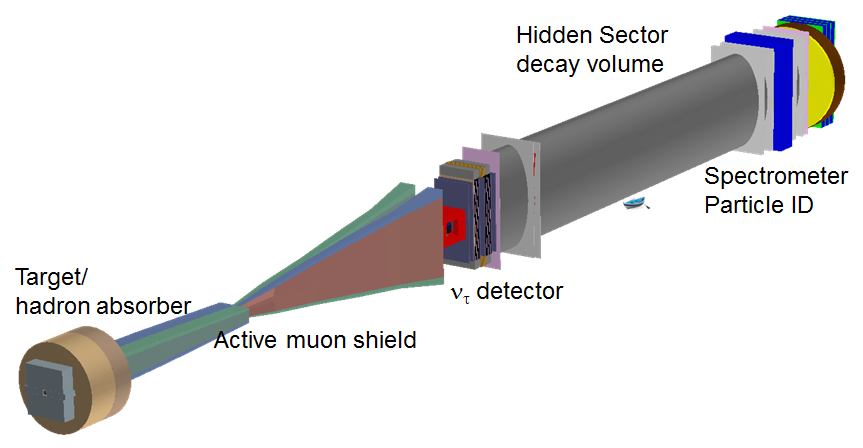
\includegraphics[width=1.78in]{pictures/ship}\\ {\tt SHiP: \href{https://arxiv.org/abs/1504.04855}{\textcolor{blue}{1504.04855}}}
	\column{0.5\textwidth}
	\centering
	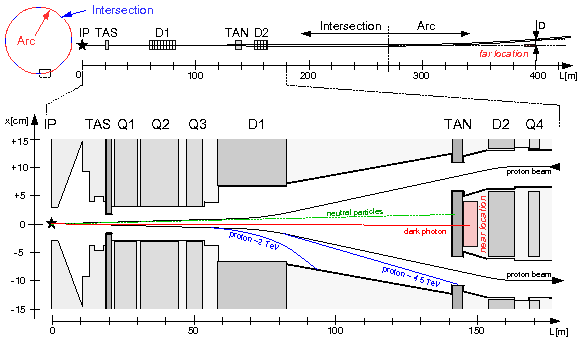
\includegraphics[width=1.6in]{pictures/faser}\\ {\tt FASER: \href{https://arxiv.org/abs/1708.09389}{\textcolor{blue}{1708.09389}}}
\end{columns}
}

\frame{
    \frametitle{Introduction - CODEX-b}
    \begin{itemize}
    \item \textbf{CO}mpact \textbf{D}etector for \textbf{EX}otics at LHC\textbf{b} (\href{https://arxiv.org/abs/1708.09395}{\textcolor{blue}{\tt 1708.09395}})
    \end{itemize}
    \vspace{0.2cm}
    \centering
    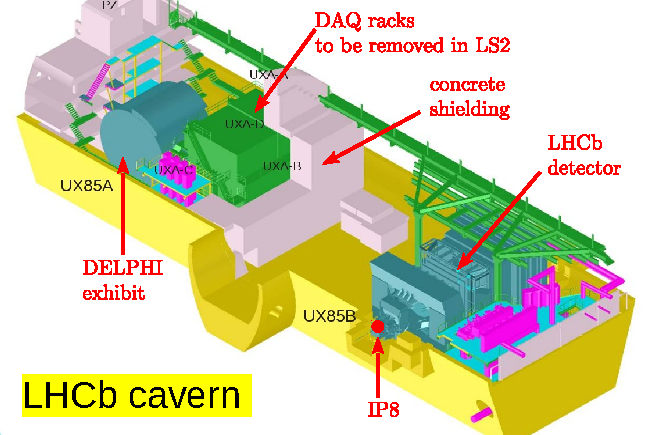
\includegraphics[width=7cm]{pictures/lhcb_cavern.pdf}
    \vspace{0.2cm}
    \begin{itemize}
    \item Move DAQ racks to surface for Run 3, instrument with tracking layers
        \vspace{0.05cm}
    \item Measure background in UXA with beam on, for physics reach studies
    \end{itemize}
}


\frame{
   \frametitle{Measurements equipment setup}
   \begin{columns}
   \column{0.5\textwidth}
   \begin{itemize}
   \item About test-bench
       \vspace{0.15cm}
   \end{itemize}
       \centering
   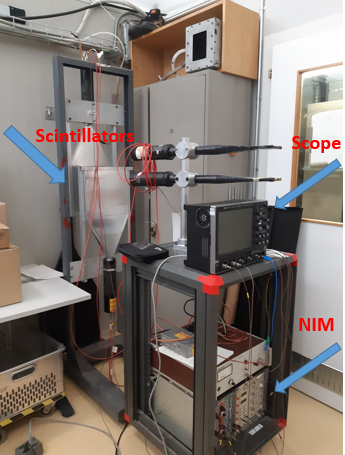
\includegraphics[width=1.9in]{pictures/Tools.png}
   \column{0.5\textwidth}
       \centering
   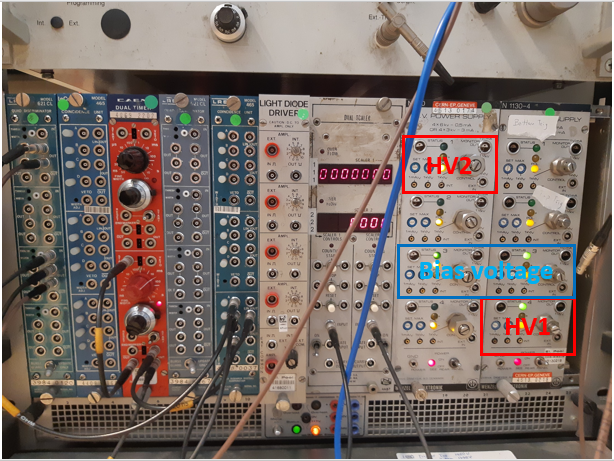
\includegraphics[width=5cm]{pictures/NIM.png}
       \vspace{0.15cm}
   \begin{itemize}
   \item Used equipments from \newline \href{https://indico.cern.ch/event/352356/contributions/1755709/attachments/697746/958057/20141202-HERSCHEL_ChallengingForUltra-HighRate.ppt}{Herschel detector}
       \vspace{0.12cm}
   \item Scintillators, PMTs, NIM, scope
   \end{itemize}
   \end{columns}
}

\frame{
   \frametitle{Scope trigger setup}
      \centering
   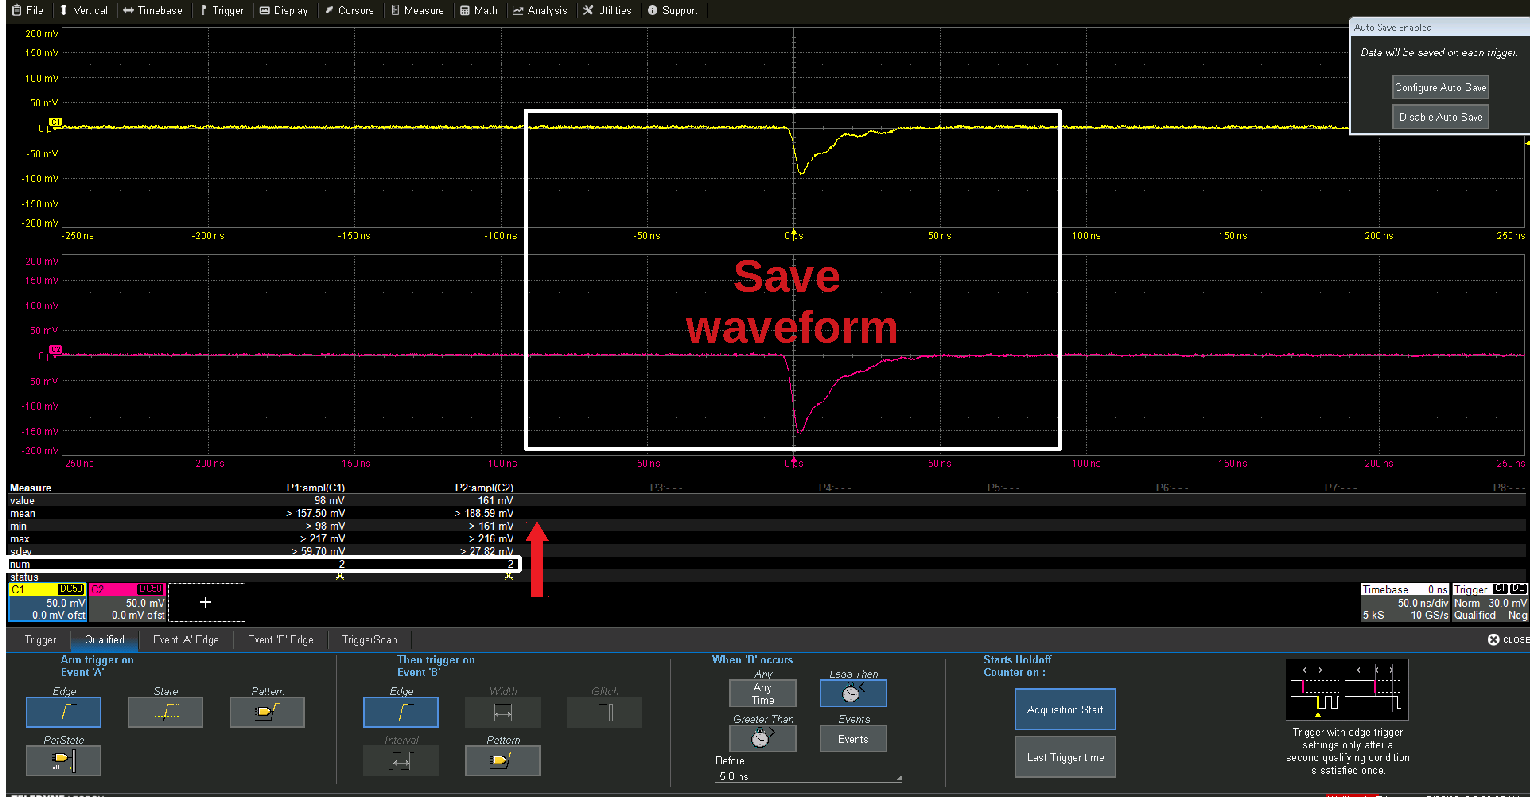
\includegraphics[width=10.5cm]{pictures/waveform.pdf}
      \vspace{0.05cm}
   \begin{itemize}
   \item Yellow - 1st scintillator (B), pink - 2nd scintillator (A)
       \vspace{0.07cm}
   \item Trigger threshold: -30 mV (falling edge)
       \vspace{0.07cm}
   \item Coincidence trigger when event A and B occur within 5 ns 
   \end{itemize}
}

\frame{
   \frametitle{Four measurement positions on D3 platform}
      \centering
   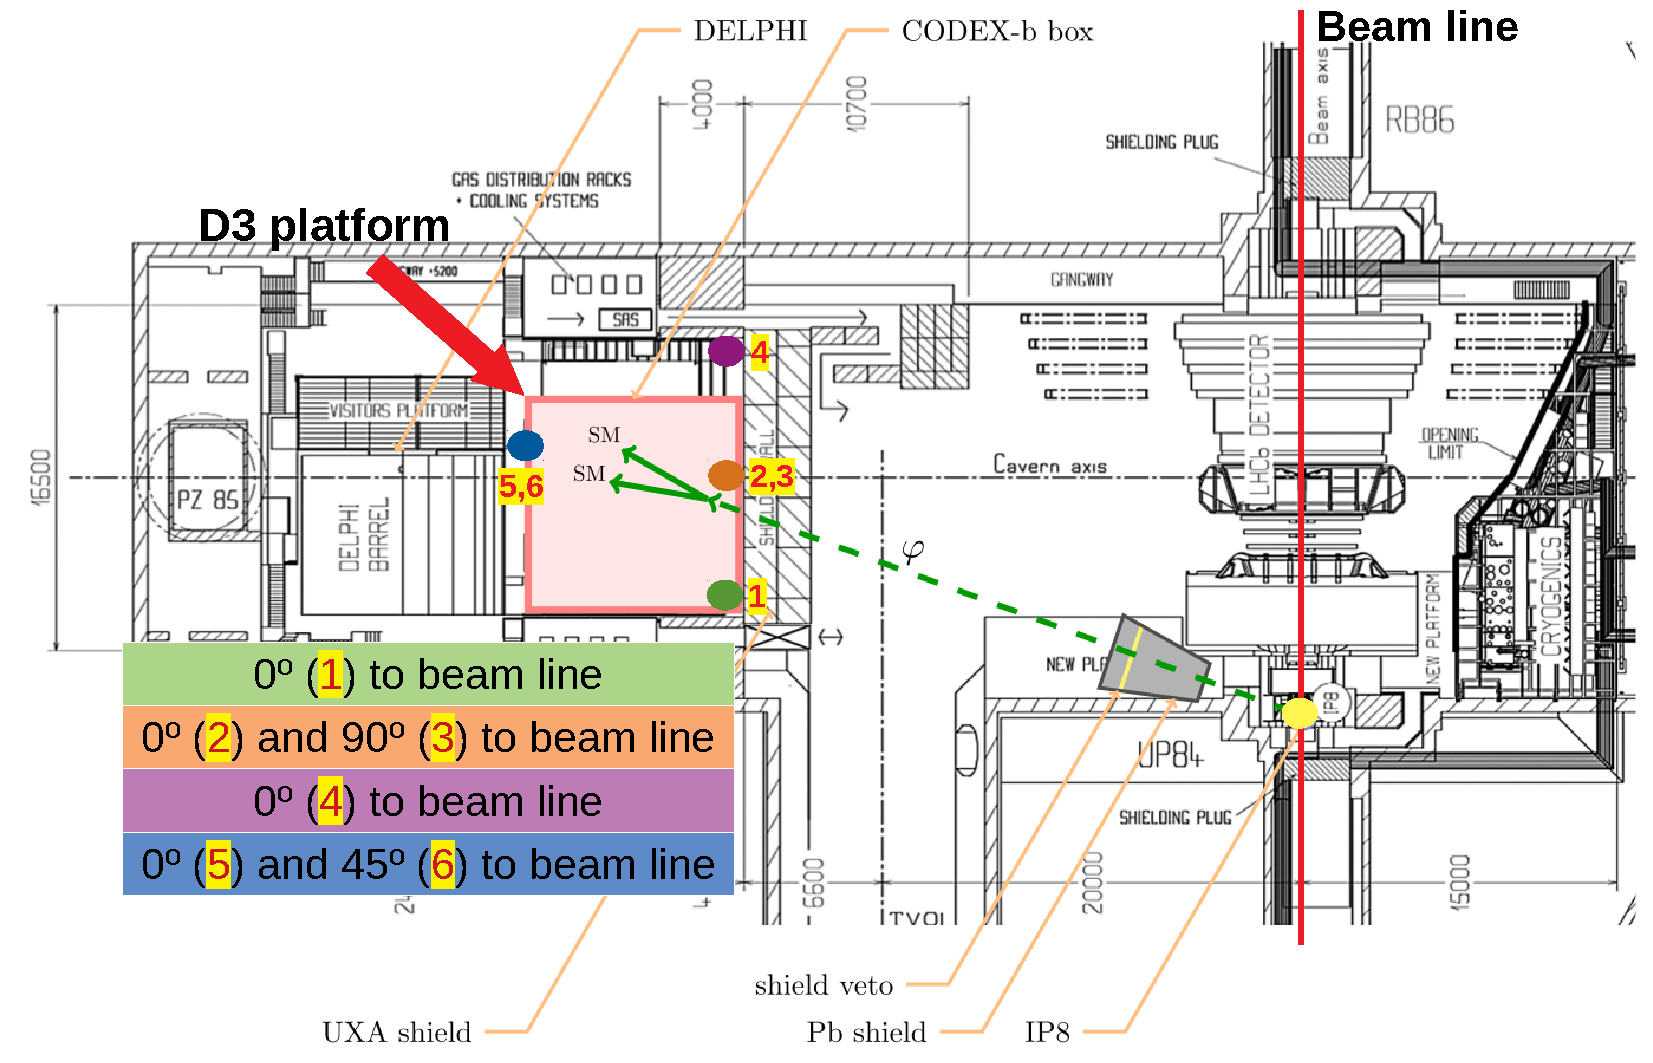
\includegraphics[width=12cm]{pictures/configuration.pdf}      
}

\frame{
   \frametitle{Measurements positions - photos}
   \begin{columns}
   \column{0.5\textwidth}
       \centering
   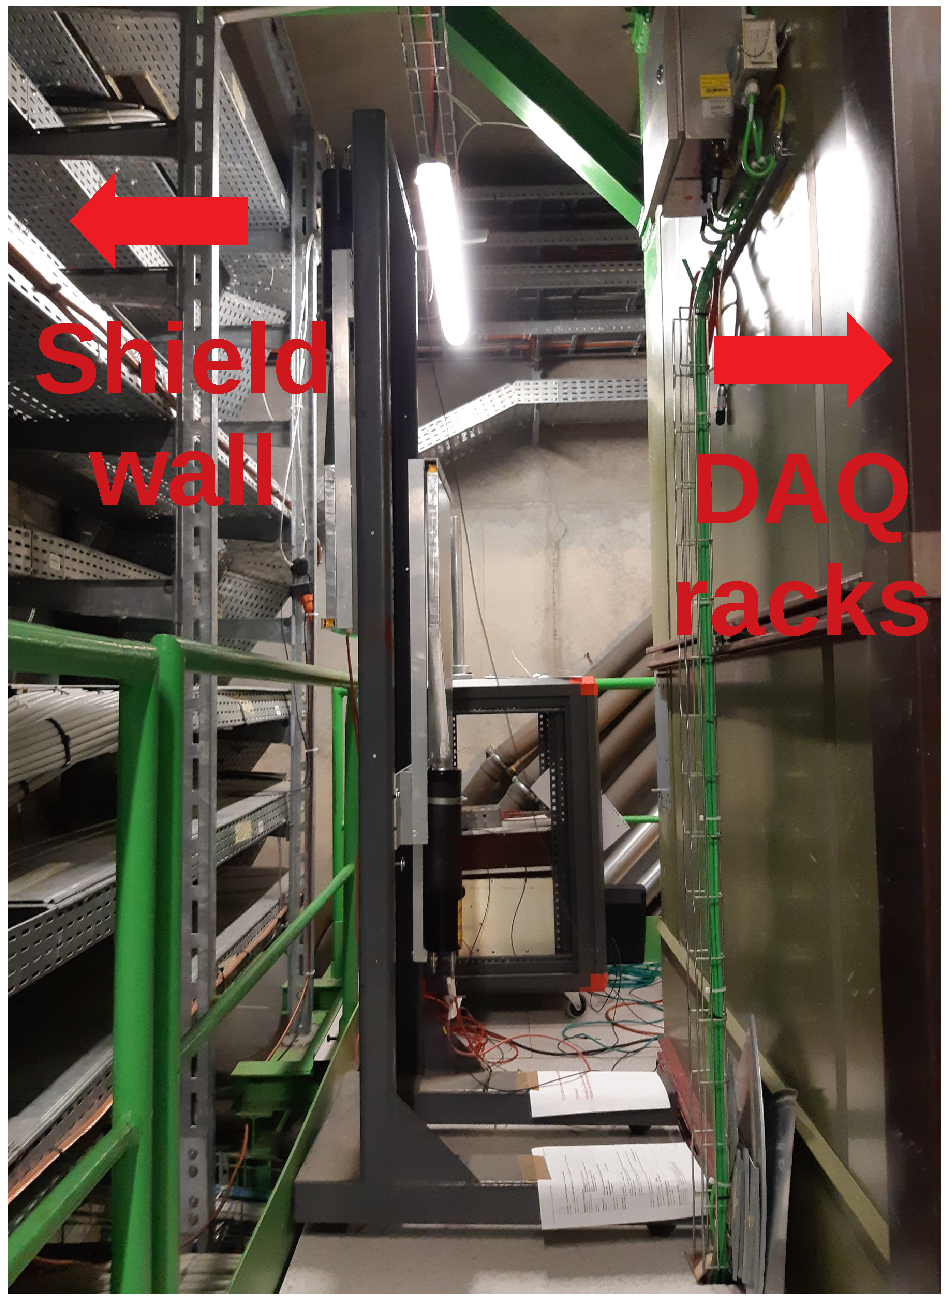
\includegraphics[width=4.5cm]{pictures/Initial.pdf}       
       \vspace{0.1cm}
   \begin{itemize}
   \item D3 back passerelle right corner
       \vspace{0.09cm}
   \item Parallel to beam line
   \end{itemize}
   \column{0.5\textwidth}
       \centering
   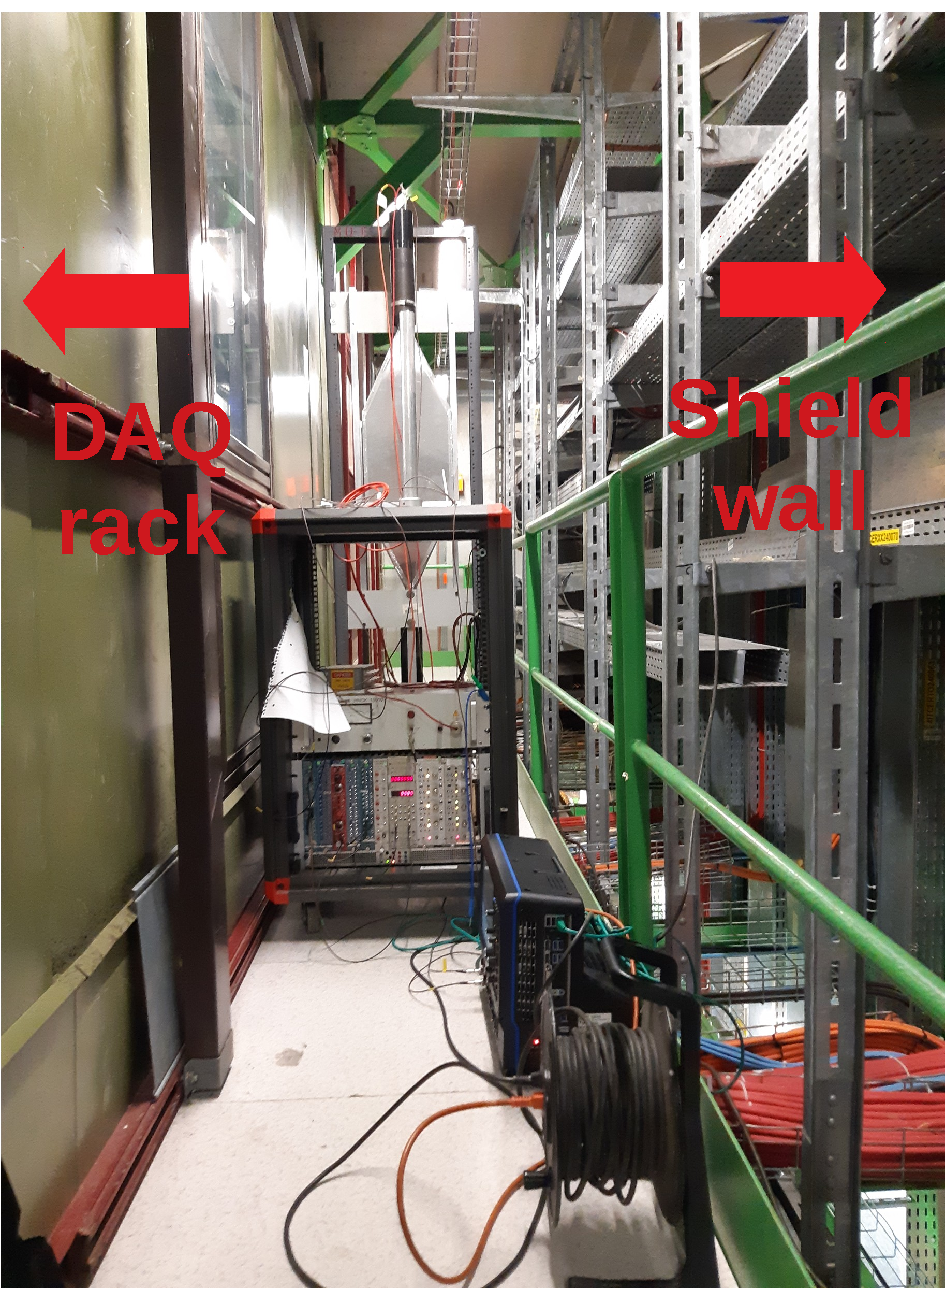
\includegraphics[width=4.5cm]{pictures/Back_central.pdf}       
       \vspace{0.1cm}
   \begin{itemize}
   \item D3 back passerelle central
       \vspace{0.09cm}
   \item Perpendicular to beam line
   \end{itemize}
   \end{columns}
}

\frame{
   \frametitle{Measurements positions - photos}
   \begin{columns}
   \column{0.5\textwidth}
       \centering
   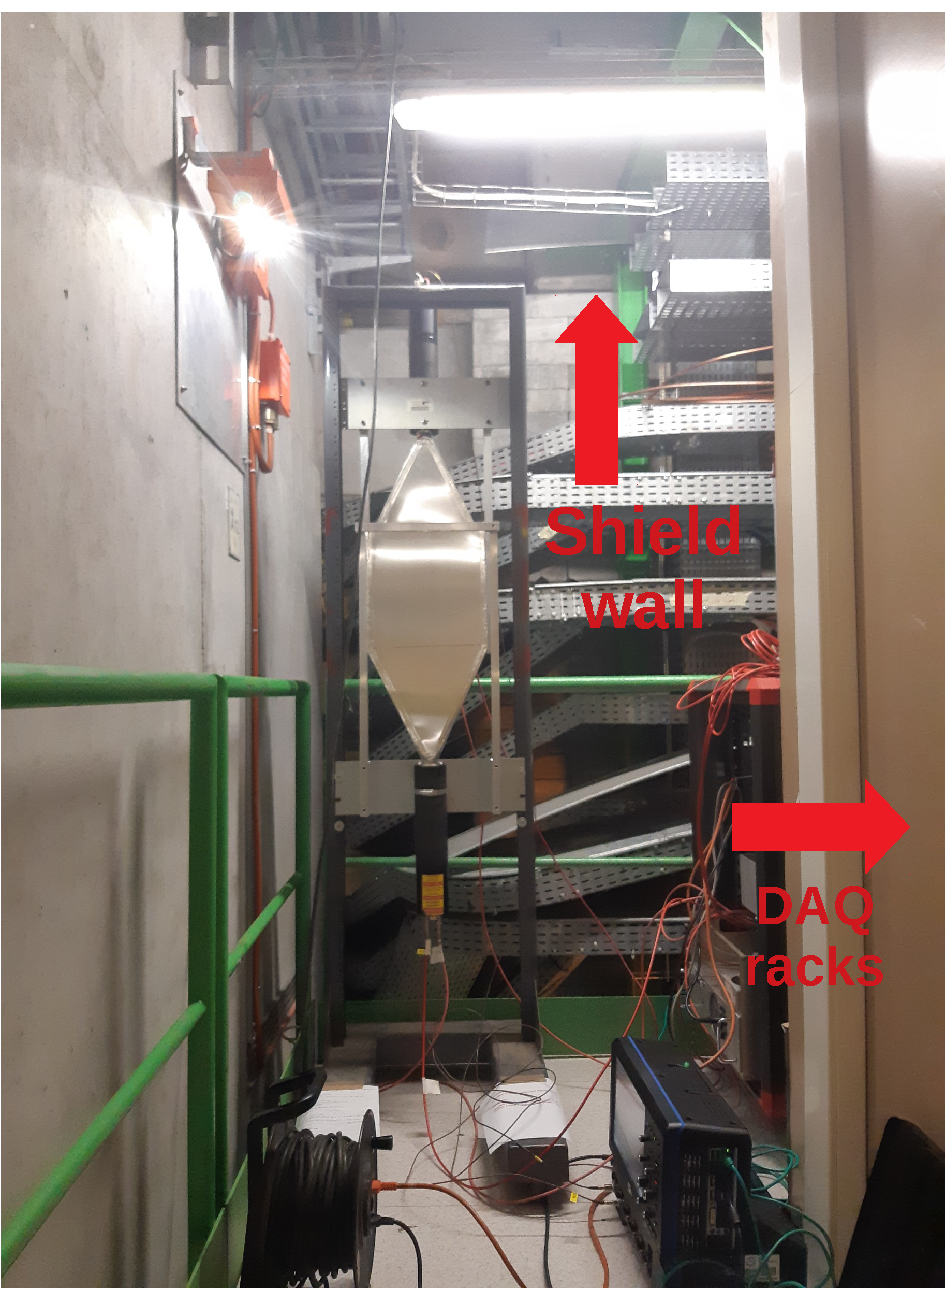
\includegraphics[width=4.5cm]{pictures/Othercorner.pdf}        
       \vspace{0.1cm}
   \begin{itemize}
   \item D3 back passerelle left corner
       \vspace{0.09cm}
   \item Parallel to beam line
   \end{itemize}
   \column{0.5\textwidth}
       \centering
   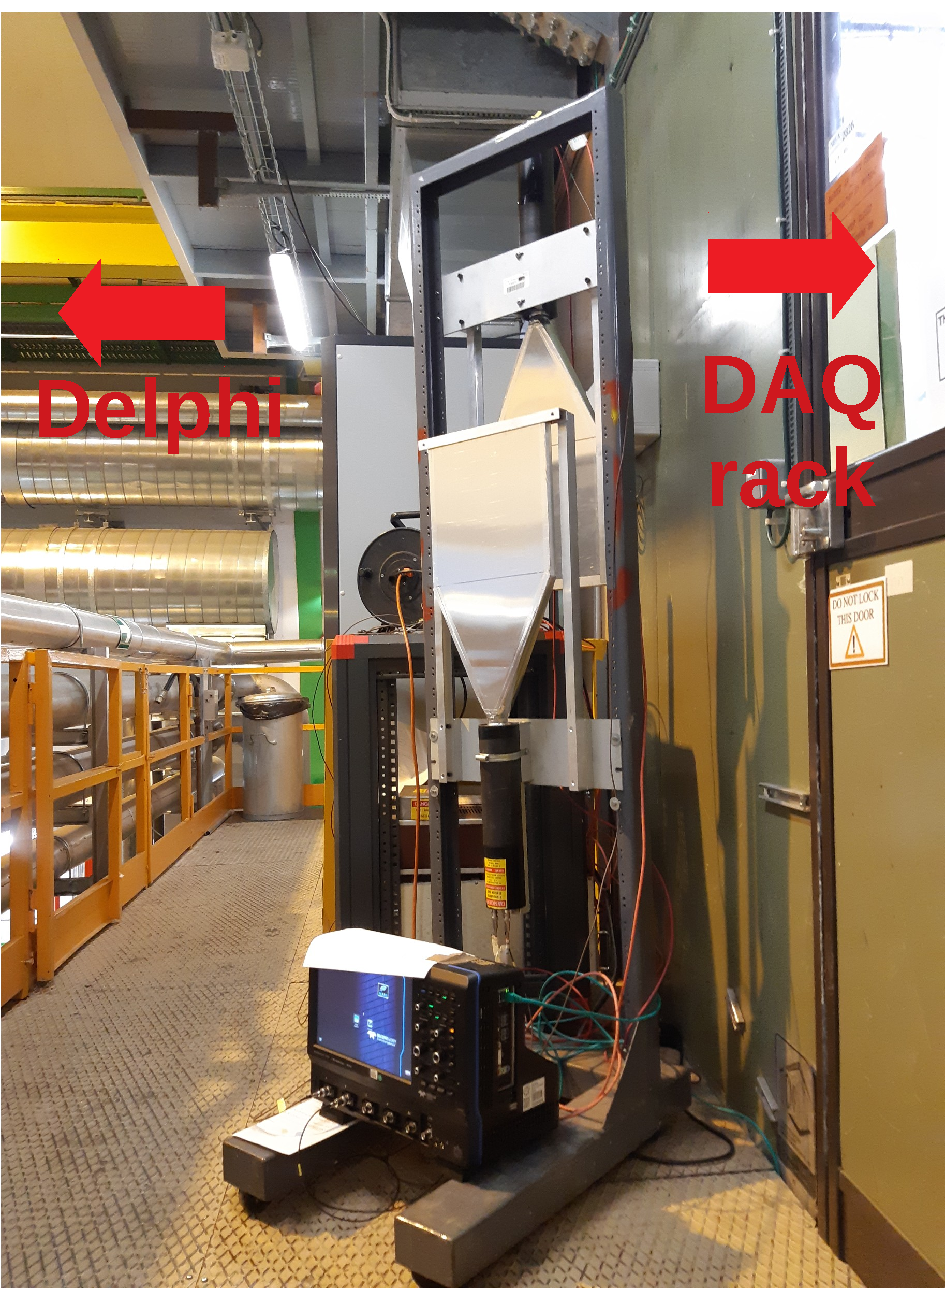
\includegraphics[width=4.5cm]{pictures/D3_front.pdf} 
       \vspace{0.1cm}
   \begin{itemize}
   \item D3 front central
       \vspace{0.09cm}
   \item 45$^\circ$ angle to beam line
   \end{itemize}
   \end{columns}
}

\frame{
   \frametitle{Global snapshot of the data}
     \vspace{-0.05cm}
     \begin{itemize}
       \item Measurement campaign spanning \textcolor{red}{17 days} in July-Aug. \textcolor{red}{52036} triggers.
       \item \textcolor{red}{6 positions/configurations} on D3 marked in blue and green, alternatingly:
     \end{itemize}
       \vspace{0.2cm}
      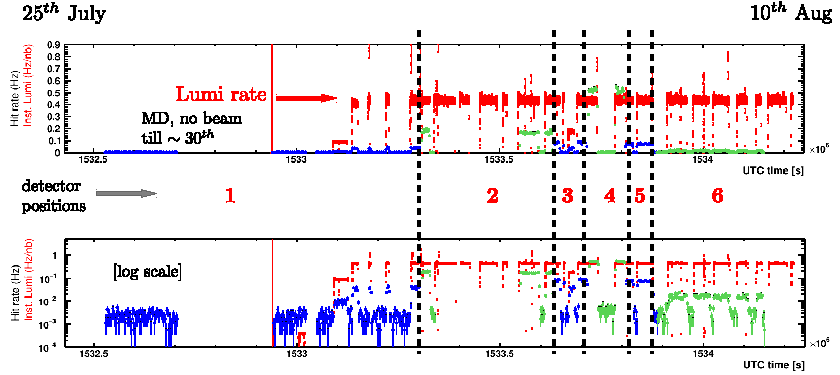
\includegraphics[width=12.4cm]{pictures/codexb_data_global.pdf}
}

\frame{
   \frametitle{Detailed features -- background rate w/o beam}
     \begin{itemize}
       \item Reminder: rate of \textcolor{blue}{$pp$} collisions + interactions is \textcolor{blue}{25~MHz} (PU=1).
       \item \textcolor{red}{Ambient} background hit rate between fills or in MD, \textcolor{red}{without beam}.
     \end{itemize}
       \vspace{0.2cm}
\begin{center}
\begin{tabular}{c|l|r}
  Position & \hspace{2cm}Description & Hit rate [mHz] \\
  \hline \hline
   P1 & shield, right corner, $\parallel$ to beam& $1.99\pm0.07$ \\ \hline
   P2 & shield, center, $\parallel$ to beam&  $2.76\pm 0.03$ \\ \hline
   P3 & shield, center, $\perp$ to beam& $ 2.26\pm 0.03$ \\ \hline
   P4 & shield, left corner, $\parallel$ to beam& $ 3.11\pm 0.03$ \\ \hline
   P5 & shield + D3 racks, center, $\parallel$ to beam& $ 1.95\pm 0.03$ \\ \hline
   P6 & shield + D3 racks, center, $45^\circ$ to beam& $ 2.22\pm $ 0.02\\ \hline
\end{tabular}
\end{center}
     \begin{itemize}
       \item Pretty consistent, \textcolor{red}{$\sim2$~mHz}, across all positions and essentially \textcolor{red}{negligible}
     \end{itemize}
}



\frame{
   \frametitle{Specific features -- rate during stable beam}
     \begin{itemize}
       \item Background hit rate during \textcolor{red}{stable beam}.
     \end{itemize}
       \vspace{0.2cm}
\begin{center}
\begin{tabular}{c|l|r}
  Position & \hspace{0.9cm}Description & Hit rate [mHz] \\
  \hline \hline
   P1 & shield, right corner, $\parallel$ to beam & $ 38.99 \pm 0.99 $\\ \hline
   P2 & shield, center, $\parallel$ to beam& $ 167.10 \pm 1.43$ \\ \hline
   P3 & shield, center, $\perp$ to beam& $ 82.81 \pm 1.55 $ \\ \hline
   P4 & shield, left corner, $\parallel$ to beam& $ 517.45 \pm 3.52 $ \\ \hline
   P5 & shield + D3 racks, center, $\parallel$ to beam& $ 73.58 \pm 1.18 $ \\ \hline
   P6 & shield + D3 racks, center, $45^\circ$ to beam& $ 15.71 \pm 0.33 $ \\ \hline
\end{tabular}
\end{center}
     \begin{itemize}
       \item Maximal rate at P4, $\sim 0.5$~Hz during beam. Calibrate simulation.
       \item The D3 racks definitely add some shielding as well (hard to simulate). 
     \end{itemize}
}

\frame{
   \frametitle{Simulation - DD4hep}
   \begin{columns}
   \column{0.5\textwidth}
   \centering
   
\includegraphics[width=5.5cm]{pictures/DD4hepLogo.png} \\
   \href{https://dd4hep.web.cern.ch/dd4hep/}{\scriptsize {\tt https://dd4hep.web.cern.ch/dd4hep/}}
   \column{0.5\textwidth}
   \begin{itemize}
   \item DD4hep is a software framework for HL-LHC upgrade 
       \vspace{0.15cm}
   \item Since CODEX-b is a new detector for HL-LHC, we chose to use it 
   \end{itemize}
   \end{columns}
   \vspace{0.35cm}
   \begin{itemize}
   \item Built CODEX-b geometry in DD4hep
       \begin{itemize}
       \item Made \textcolor{red}{hierachy system} (envelope $\rightarrow$ super station $\rightarrow$ station $\rightarrow$ layer)
           \vspace{0.1cm}
       \item Tested with a $\mu$ particle gun
           \vspace{0.1cm}
       \item Checked \textcolor{red}{energy deposits and positions} of CODEX-b hits
       \end{itemize}
   \vspace{0.2cm}
   \item Tested with \textcolor{red}{MinBias} (standalone Gauss) $\to$ HepMC format $\to$ DDG4
   \item Hits read out using DD4hep plugin, checked that they look reasonable
   \end{itemize}
}

\frame{
   \frametitle{Detector geometry in DD4hep}
   \begin{columns}
   \column{0.5\textwidth}
   \centering
       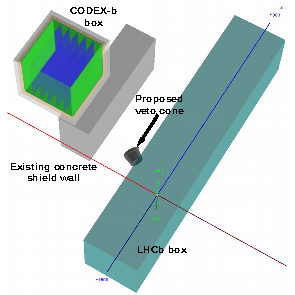
\includegraphics[width=6.5cm]{pictures/CODEXbBigGeo.pdf}
   \column{0.5\textwidth}
   \begin{itemize}
   \item Veto cone
       \vspace{0.15cm}
       \begin{itemize}
       \item {\footnotesize Two Pb absorbers}
       \vspace{0.1cm}
       \item {\footnotesize One active Si shield layer}
       \end{itemize}
   \vspace{0.2cm}
   \item Concrete shield wall
       \vspace{0.15cm}
       \begin{itemize}
       \item {\footnotesize 3.2 m thickness}
       \vspace{0.1cm}
       \item {\footnotesize Block most particles from 
       \newline \textit{pp} collisions}
       \end{itemize}
   \vspace{0.2cm}
   \item CODEX-b box
       \vspace{0.15cm}
       \begin{itemize}
       \item {\footnotesize Consists of two types of stations}
       \end{itemize}
   \end{itemize}
   \end{columns}
}

\frame{
   \frametitle{Detector geometry in DD4hep - Zoom}
   \begin{itemize}
   \item Geometry was taken from \href{https://arxiv.org/abs/1708.09395}{\textcolor{blue}{\tt 1708.09395}} (not final!)
   \end{itemize}
   \begin{columns}
   \column{0.5\textwidth}
   \centering
       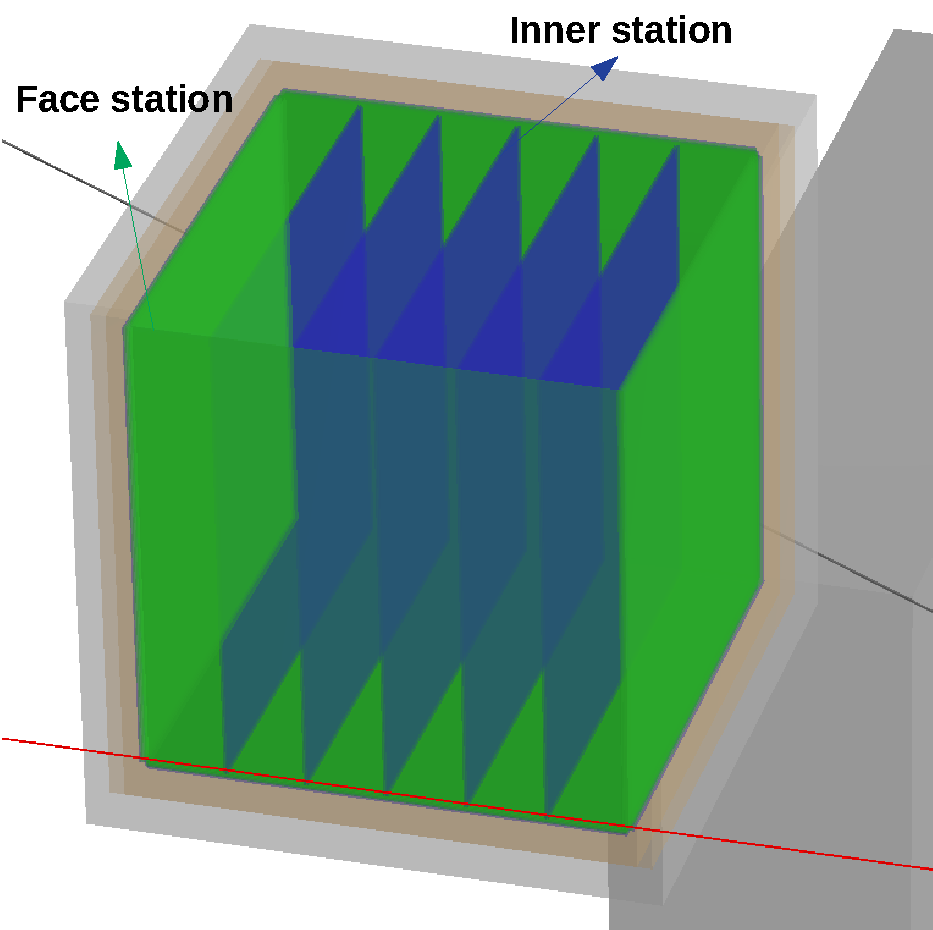
\includegraphics[width=6.2cm]{pictures/ZoomVersion.pdf}
   \column{0.5\textwidth}
   \begin{itemize}
   \item Inner station (x5)
       \vspace{0.15cm}
       \begin{itemize}
       \item {\footnotesize Silicon tracker}
       \vspace{0.1cm}
       \item {\footnotesize 3 layers of 10 x 10 $m^{2}$ size 
       \newline and 2 cm thickness}
       \vspace{0.1cm}
       \item {\footnotesize Distance between layers is 4 cm}
       \end{itemize}
   \vspace{0.2cm}
   \item Face station (x6)
       \vspace{0.15cm}
       \begin{itemize}
       \item {\footnotesize Silicon tracker}
       \vspace{0.1cm}
       \item {\footnotesize 6 layers of 10  x 10 $m^{2}$ size 
       \newline and 2 cm thickness}
       \vspace{0.1cm}
       \item {\footnotesize Distance between layers is 4 cm}
       \end{itemize}
   \end{itemize}
   \end{columns}
}

\frame{
   \frametitle{DD4hep simulation with minbias events - CODEX-b}
   \begin{itemize}
   \item 13\tev minbias events with \textcolor{red}{existing shield \textbf{removed}} 
   \end{itemize}
   \vspace{0.2cm}
   \centering
       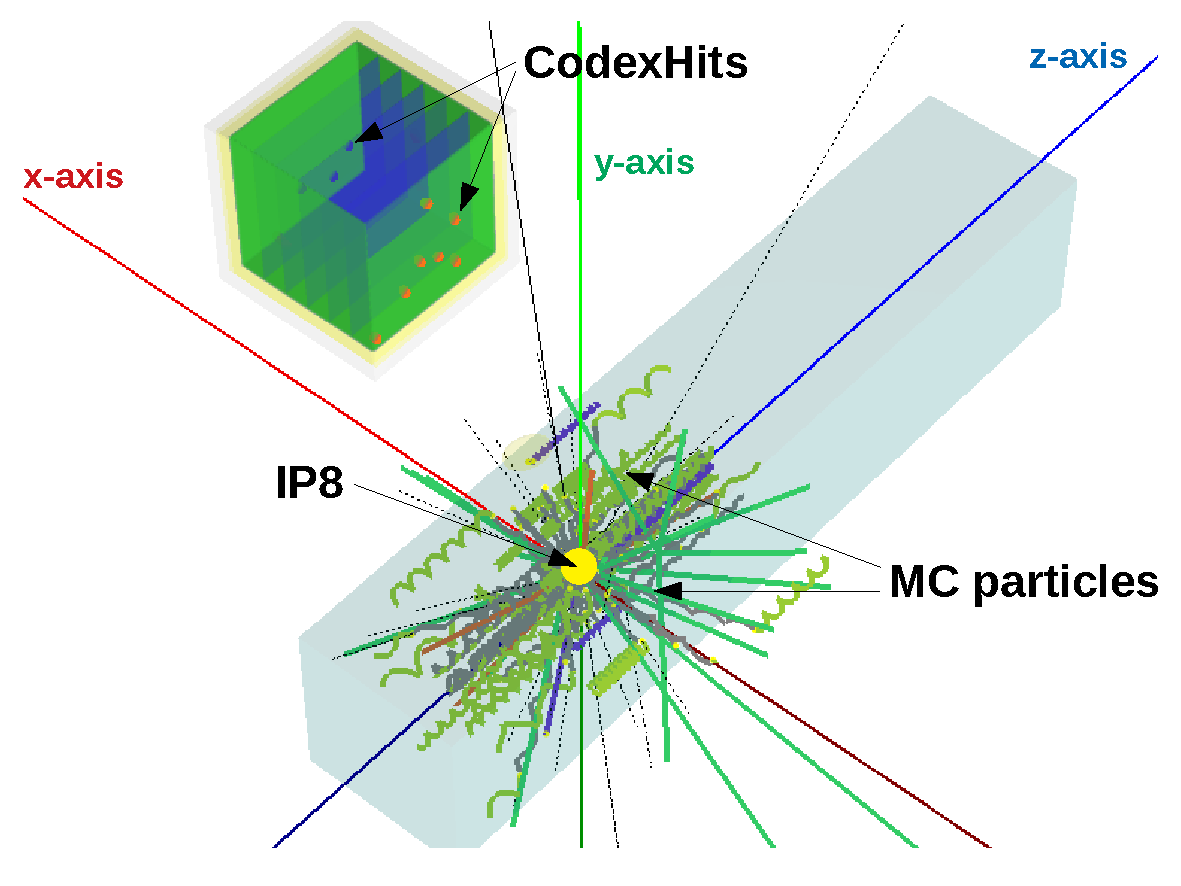
\includegraphics[width=9cm]{pictures/Minbias.pdf}
}

\frame{
   \frametitle{DD4hep simulation with minbias events - scintillators}
   \vspace{-0.2cm}
   \begin{itemize}
   \item \textcolor{red}{32k events}, generated in \textcolor{red}{4$\pi$}, using {\tt minbias.dec}, \textcolor{red}{no hits!}
   \end{itemize}
   \centering
       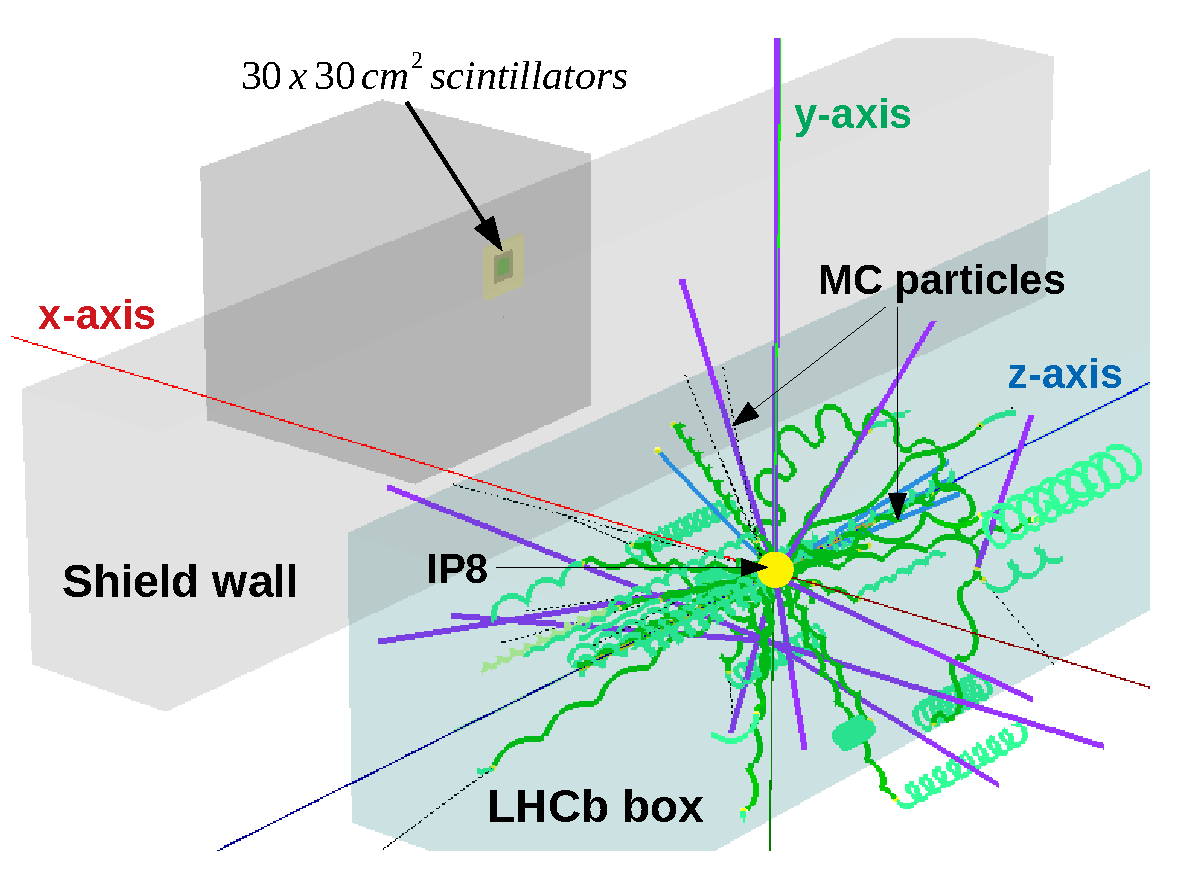
\includegraphics[width=8.5cm]{pictures/Scint.pdf}
   \vspace{0.05cm}
   \begin{itemize}
   \item New dec file with generator cuts is work in progress
   \end{itemize}

}

\frame{
   \frametitle{Summary and future plan}
   \begin{itemize}
   \item Very \textcolor{red}{successful} background measurement \textcolor{red}{campaign} at D3
       \vspace{0.42cm}
   \item Background \textcolor{red}{rate} just behind shield wall around \textcolor{red}{0.5~Hz} over \textcolor{red}{900cm$^{2}$}
       \vspace{0.42cm}
   \item \textcolor{red}{DD4hep-based} \textcolor{red}{simulation} fully tested both measurement and CODEX-b configurations
       \vspace{0.42cm}
   \item Working on more efficient MC generation in Gauss \textcolor{red}{w/ generator cuts}
       \vspace{0.42cm}
   \item {Presented at \href{https://indico.cern.ch/event/722726/contributions/3102422/attachments/1699623/2736731/talk8.pdf}{\textcolor{blue}{Run meeting}} on 10/08}
       \vspace{0.42cm}
   \item Once simulation is ready, finalize the \textcolor{red}{internal note}
   \end{itemize}
}

\frame{
   \frametitle{Acknowledgements}
   \begin{itemize}
   \item My summer student supervisors: Biplab Dey, Victor Coco
       \vspace{0.2cm}
   \item DD4hep developer: Markus Frank
       \vspace{0.2cm}
   \item Equipments from Herschel detector: Heinrich Schindler, Raphael Dumps
       \vspace{0.2cm}
   \item Theoretical parts: Vladimir Gligorov
       \vspace{0.2cm}
   \item At the pit: Tengiz Kvaratskheliya
   \end{itemize}
   \vspace{0.3cm}
   \pause
       \centering
       {\Large Thanks to LHCb for a wonderful experience !}
}

\frame{
    \centering
    {\Huge \textbf{Thank you}}
}

